\documentclass[conference]{IEEEtran}
\IEEEoverridecommandlockouts

% More defined colors
\usepackage[table,xcdraw]{xcolor}
\usepackage[spanish,es-tabla]{babel}
\usepackage{lipsum}
\usepackage{cite}

\usepackage{booktabs}
\usepackage[toc,page]{appendix}
\usepackage{fancyhdr}
\usepackage{amssymb} %PARA SÍMBOLOS GRIEGOS Y MATEMÁTICOS
\usepackage{gensymb}
\usepackage{tabularx} 
% Required package
\usepackage{tikz}
\usetikzlibrary{positioning}
\usepackage{float}
\usepackage{caption}
\usepackage{cite}
\usepackage{amsmath,amssymb,amsfonts}
\usepackage{algorithmic}
\usepackage{graphicx}
\usepackage{textcomp}
\usepackage{mathtools}  
\usepackage{multirow}
\def\BibTeX{{\rm B\kern-.05em{\sc i\kern-.025em b}\kern-.08em
    T\kern-.1667em\lower.7ex\hbox{E}\kern-.125emX}}
\usepackage[spanish]{babel}
\usepackage{hyperref}
\selectlanguage{spanish}


\begin{document}

\title{Proyecto\\ Red LoRa de Múltiples Nodos de Sensores Inalámbricos y Gateway para \\ Aplicaciones Agrícolas}
\renewcommand{\figurename}{Fig.} 

\author{
\IEEEauthorblockN{...}
\IEEEauthorblockA{\textit{Tecnológico de Costa Rica} \\
\textit{Escuela de Ingeniería Electrónica}\\
Sede Cartago \\
...@estudiantec.cr \\
...\\}

\and

\IEEEauthorblockN{Andrés Rojas Barboza}
\IEEEauthorblockA{\textit{Tecnológico de Costa Rica} \\
\textit{Escuela de Ingeniería Electrónica}\\
Sede Cartago \\
andyrb506@estudiantec.cr \\
2019164947\\}

\and

\IEEEauthorblockN{Hertzel Caballero Rojas}
\IEEEauthorblockA{\textit{Tecnológico de Costa Rica} \\
\textit{Escuela de Ingeniería Electrónica}\\
Sede Cartago \\
2019063854@estudiantec.cr \\
2019063854\\}

}

\maketitle

\begin{abstract}
Este documento presenta los conceptos de LoRa, APRS y el PNAF con el fin de diseñar y analizar una red basada en tecnología LoRa para aplicaciones agrícolas. El diseño de la red basada en tecnología LoRa para aplicaciones agrícolas implica unos nodos sensores que están pensados para medir diversos parámetros ambientales. Estos nodos son capaces de monitorear la humedad del suelo a diferentes profundidades (20, 40 y 60 cm), la temperatura y humedad ambiental, la intensidad de luz, y la presencia de lluvia. Además, se comenta que para el procesamiento y transmisión de datos, se utilizaron los microcontroladores Heltec LoRa ESP32 y ATmega2560. Se analiza los resultados arrojados por ese diseño los cuales son que los sensores lograron una precisión superior al 90\% en comparación con instrumentos estándar, el gateway fue capaz de transmitir los datos recolectados a la nube cada 15 segundos. En cuanto con el error promedio de medición de humedad se valoró en un 1.3\% a 9\%, y de la medición de la luz de 11\%. Se concluye que la integración de APRS y LoRa es altamente beneficiosa para el control de la agricultura por su bajo consumo energético y largas dintancias.
   
\end{abstract}
\begin{IEEEkeywords}
APRS, LoRa, PNAF, sensores, humedad, luz, temperatura.
\end{IEEEkeywords}

\section{\textbf{Introducción}}
En el contexto de las comunicaciones inalámbricas, la implementación de redes de sensores agrícolas utilizando tecnología LoRa representa una evolución práctica y eficiente dentro del marco del APRS y sus variantes modernas. Al integrar LoRa con sistemas de recolección y transmisión de datos ambientales, como se plantea en este documento, se aprovechan las ventajas de su bajo consumo energético y su largo alcance para aplicaciones del Internet de las Cosas (IoT). 

\vspace{2mm}

Este enfoque es particularmente relevante en entornos rurales donde las redes tradicionales presentan limitaciones. La arquitectura propuesta, basada en múltiples nodos sensores inalámbricos y un gateway LoRa conectado a la nube, demuestra cómo este tipo de soluciones pueden complementar o incluso superar a sistemas tradicionales como APRS en ciertos escenarios de monitoreo ambiental. Además, la operación de estos sistemas dentro de bandas de frecuencia no licenciadas exige una comprensión clara del marco regulatorio local, como el Plan Nacional de Atribución de Frecuencias (PNAF) en Costa Rica, que garantiza el uso ordenado y eficiente del espectro radioeléctrico en aplicaciones de interés nacional.

\vspace{2mm}

Bajo ese orden de ideas, en este documento en la sección de Estado del Arte se exploran los fundamentos de APRS, su integración con Internet a través de APRS-IS, y el uso de distintos protocolos de transmisión, incluyendo AX.25 y LoRa. Posteriormente, se revisa el Plan Nacional de Atribución de Frecuencias (PNAF) en Costa Rica, así como sus respectivas regulaciones.

\vspace{2mm}

Luego, en la sección de Metodología, esta sección se planea abordar la organización de equipo y un diagrama de Gantt que muestre el trabajo realizado en sus respectivas fechas. Además, se pretende explorar y analizar un diseño de red de nodos sensores inalámbricos multiambientales con gateway LoRa con el fin de valorar si estos son eficientes a la hora de recolectar datos ambientales en tiempo real con bajo costo.  

\vspace{2mm}

Después, en la sección de Implementación, se pretende realizar diagramas hasta tercer nivel con el fin de describir los componentes principales de la red de nodos sensores inalámbricos multiambientales con gateway LoRa.


\section{\textbf{Estado del Arte}}

En esta sección se pretende brindar al lector un contexto más amplio sobre los conceptos mencionados brevemente en la introducción.

\vspace{2mm}

\begin{center}
\textbf{\large APRS}
\end{center}

Un Sistema Automático de Reporte de Paquetes (APRS) es una comunicación bidireccional digital en tiempo real entre todos los miembros de una red que comparten información. 

\newpage

Esto implica que cualquier cosa de ``valor'' en el área local será capturada por el dispositivo APRS, y al mismo tiempo, este también estará enviando información de ``valor'' a la red \cite{APRS}. 

\vspace{2mm}

Los datos de los dispositivos APRS son típicamente transmitidos a una frecuencia compartida y son repetidos por estaciones de relé para consumo local distribuido. Todos los datos se ingresan a un sistema de Internet APRS (APRS-IS) vía un receptor conectado a Internet (IGate), y se distribuyen para acceso por todos los usuarios de la red. Pueden servir para telemetría, transmisión en redes LAN, GPS, etc.

\vspace{2mm}

Existe una gran variedad de protocolos de comunicación. La elección del protocolo depende de la aplicación específica. El más usado es el protocolo AX.25, derivado de X.25 pero adaptado para radioaficionados. Sin embargo, no es el único protocolo disponible.

\vspace{2mm}

\subsection*{\textbf{Protocolos de comunicación en APRS}}

\begin{enumerate}
    \item \textbf{AX.25}  
    \begin{itemize}
        \item Soporta comunicación a través de Packet Radio.  
        \item Funciona con módems AFSK a 1200 bps y enlaces VHF (30 a 300 MHz, [144.39 MHz en Costa Rica]).
    \end{itemize}

    \item \textbf{APRS-IS}  
    \begin{itemize}
        \item Integra APRS con Internet.  
        \item Utiliza TCP/IP para conectar las estaciones APRS, IGates y servidores APRS.
    \end{itemize}

    \item \textbf{LoRa}  
    \begin{itemize}
        \item Se usa cuando se quiere comunicación a larga distancia con baja velocidad de transmisión de datos y cuando la aplicación requiere bajo consumo de energía.
    \end{itemize}
\end{enumerate}

\vspace{1em}
\begin{center}
\textbf{\large LoRa}
\end{center}

LoRa es una técnica de modulación para transmisiones eléctricas sin hilos derivada de Espectro Expandido en Chirps. Esto significa que utiliza una señal sinusoidal moduladora cuya frecuencia no es fija, sino que oscila en un rango de frecuencias. Esto la hace robusta contra interferencias en comunicaciones a larga distancia \cite{LoRa}.

\vspace{2mm}

LoRa es ideal para aplicaciones en las que se desea transmitir conjuntos de datos pequeños o con baja tasa de transmisión. Ejemplos incluyen:

\begin{itemize}
    \item Aplicaciones de agricultura y riego, donde se requiere transmitir instrucciones a larga distancia y tomar decisiones en espacios abiertos con baja supervisión.
    \item Soluciones en ciudades inteligentes, como logística de transporte, medición de variables ambientales y sistemas de seguridad.
    \item Monitorización de infraestructuras: puentes, edificios, supervisión de paneles solares, etc.
\end{itemize}

\newpage

Los datos pueden ser transmitidos a distancias más largas en comparación con tecnologías como Bluetooth o WiFi. Estas características la hacen ideal para aplicaciones IoT y censado en dispositivos que deben ser dejados en operación sin supervisión durante largos periodos. LoRa opera en frecuencias libres de VHF. En el caso de Costa Rica, abarca las frecuencias de 902 MHz a 928 MHz.

\vspace{2mm}

Existen diversos módulos disponibles en el mercado con soporte para LoRa. Por ejemplo, el \textbf{ESP32 Doit}, una tarjeta de desarrollo creada por DOIT, que puede usarse con el módulo \textbf{ESP32-WROOM-32}. Este módulo permite comunicación WiFi y Bluetooth con frecuencias de reloj ajustables en el rango de 80 MHz a 240 MHz.

\vspace{2mm}

\begin{center}
\textbf{\large PNAF}
\end{center}

El \textbf{Plan Nacional de Atribución de Frecuencias (PNAF)} es un instrumento que permite la regulación nacional de manera óptima, racional, económica y eficiente del espectro radioeléctrico nacional. Su objetivo es satisfacer oportuna y adecuadamente las necesidades de frecuencias para el desarrollo de redes de telecomunicaciones y responder eficientemente a la demanda de segmentos de frecuencias para redes que hagan uso del espectro radioeléctrico. Para ello, se promueve el uso de tecnologías que optimicen su utilización, conforme al marco legal y reglamentario vigente y los acuerdos internacionales ratificados por Costa Rica \cite{PNAF}.

\vspace{0.1mm}

\subsection*{Clasificación del espectro radioeléctrico:}

\begin{itemize}
    \item \textbf{Uso comercial}: Para la prestación de servicios de telecomunicaciones disponibles al público a cambio de una contraprestación económica.
    \item \textbf{Uso no comercial}: Para operaciones de carácter temporal, experimental, científico, servicios de radiocomunicación privada, banda ciudadana, radioaficionados o redes de telemetría de instituciones públicas.
    \item \textbf{Uso oficial}: Para establecer las comunicaciones de las instituciones del Estado, con uso exclusivo para el servicio asignado y no comercial.
    \item \textbf{Uso para seguridad, socorro y emergencia}: Para radionavegación, seguridad aeronáutica, marítima y otros servicios de ayuda.
    \item \textbf{Uso libre}: No requiere concesión, autorización o permiso, estando sujeto a las características técnicas establecidas en el Adendum VII del PNAF.
\end{itemize}

\vspace{2mm}

\section{\textbf{Metodología}}
En esta sección se encuentra tanto la organización que se tuvo en el equipo, así como la red basada en tecnología LoRa para aplicaciones agrícolas basada en el informe \cite{paper}.

\newpage

\subsection*{Organización del equipo:}

Para la elaboración de este proyecto, se empezó por realizar un Diagrama de Gantt con el fin de poder tener una guía de las entregas de avances y de las asignaciones de cada miembro de trabajo.

\vspace{2mm}

\begin{figure}[H]
    \centering
    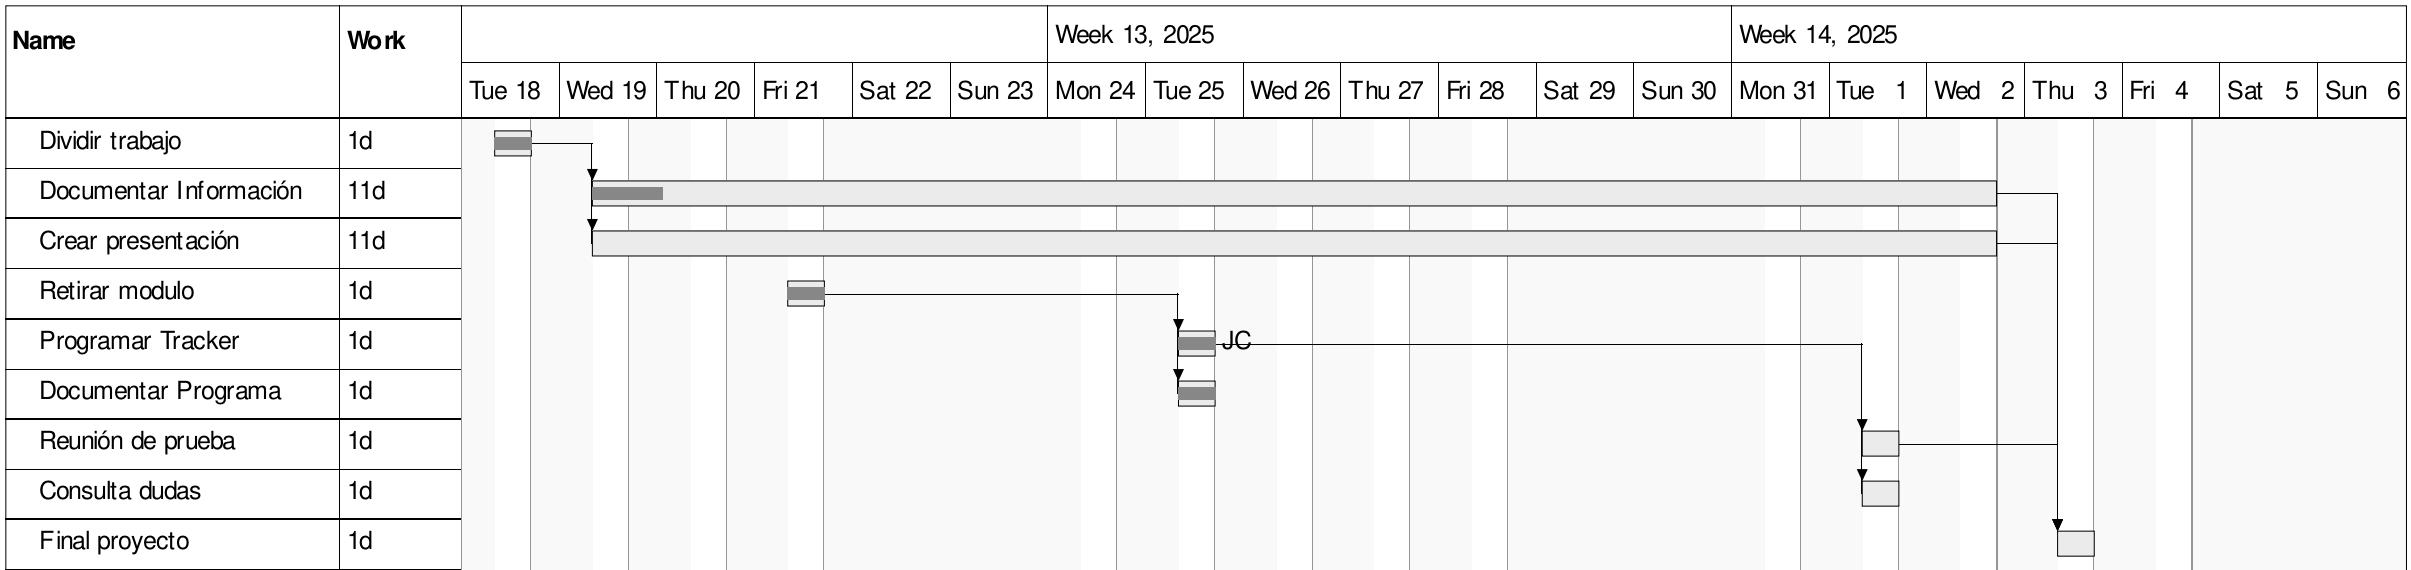
\includegraphics[width = 1\linewidth]{Imagenes/Diagrama de Gantt.jpg}
    \caption{Diagrama de Gantt del equipo de trabajo}
    \label{fig:Gantt}
\end{figure}


\subsection*{Red basada en tecnología LoRa para aplicaciones agrícolas:}

\vspace{2mm}

El diseño de la red LoRa para aplicaciones en zonas agrícolas incluye múltiples nodos sensores ambientales LoRa (como se muestra en la Fig. \ref{fig:lora_network}, compuestos por un número $n$ de nodos sensores), microcontroladores, una pasarela LoRa y almacenamiento en la nube.

\vspace{2mm}

\begin{enumerate}
    \item \textbf{Sección de hardware:} Cada nodo sensor ambiental recopila datos del entorno en distintas áreas agrícolas. Posteriormente, transmite los datos de forma inalámbrica a una frecuencia de 925.2 MHz hacia una Raspberry Pi, que actúa como unidad central de procesamiento en la pasarela LoRa. Finalmente, los datos recopilados son enviados desde la pasarela hacia el almacenamiento en la nube utilizando WiFi en la banda de 2.4 GHz.
    
    \item \textbf{Sección de software:} El diseño del software se segmenta en tres partes, dependiendo del tipo de microcontrolador y del almacenamiento en la nube. Los microcontroladores Heltec LoRa y ATmega2560 utilizan el entorno de desarrollo Arduino IDE. La Raspberry Pi opera con el sistema operativo Raspbian. Para la gestión de la red LoRaWAN, se utiliza ChirpStack, una plataforma de código abierto. Adicionalmente, se emplea Grafana como panel de control gráfico para la visualización y análisis de los datos ambientales.
\end{enumerate}

\section{\textbf{Implementación}}

\vspace{2mm}

Con el objetivo de monitorear de forma eficaz la migración y el comportamiento de animales en peligro de extinción, se ha desarrollado un sistema de rastreo robusto y energéticamente eficiente. Esta solución integra tecnologías como GPS, LoRa y el protocolo APRS, permitiendo la transmisión en tiempo real de datos de posición, velocidad y temperatura. En la Fig.~\ref{fig:tracker_diagram} se muestra el diagrama de bloques que representa los principales componentes del sistema de rastreo, diseñado para funcionar de manera autónoma en entornos remotos y de difícil acceso. Esta implementación se basa en la aplicada en el ejemplo \cite{paper}.

\vspace{2mm}

El diagrama describe los distintos módulos que conforman el sistema, incluyendo la fuente de energía, la adquisición y procesamiento de datos, el módulo de transmisión y el sistema de visualización remota. A continuación, se detalla cada uno de estos bloques y sus respectivas funciones internas, los cuales trabajan en conjunto para proporcionar un monitoreo confiable y preciso de las especies rastreadas.

\vspace{2mm}

\begin{figure}[H]
    \centering
    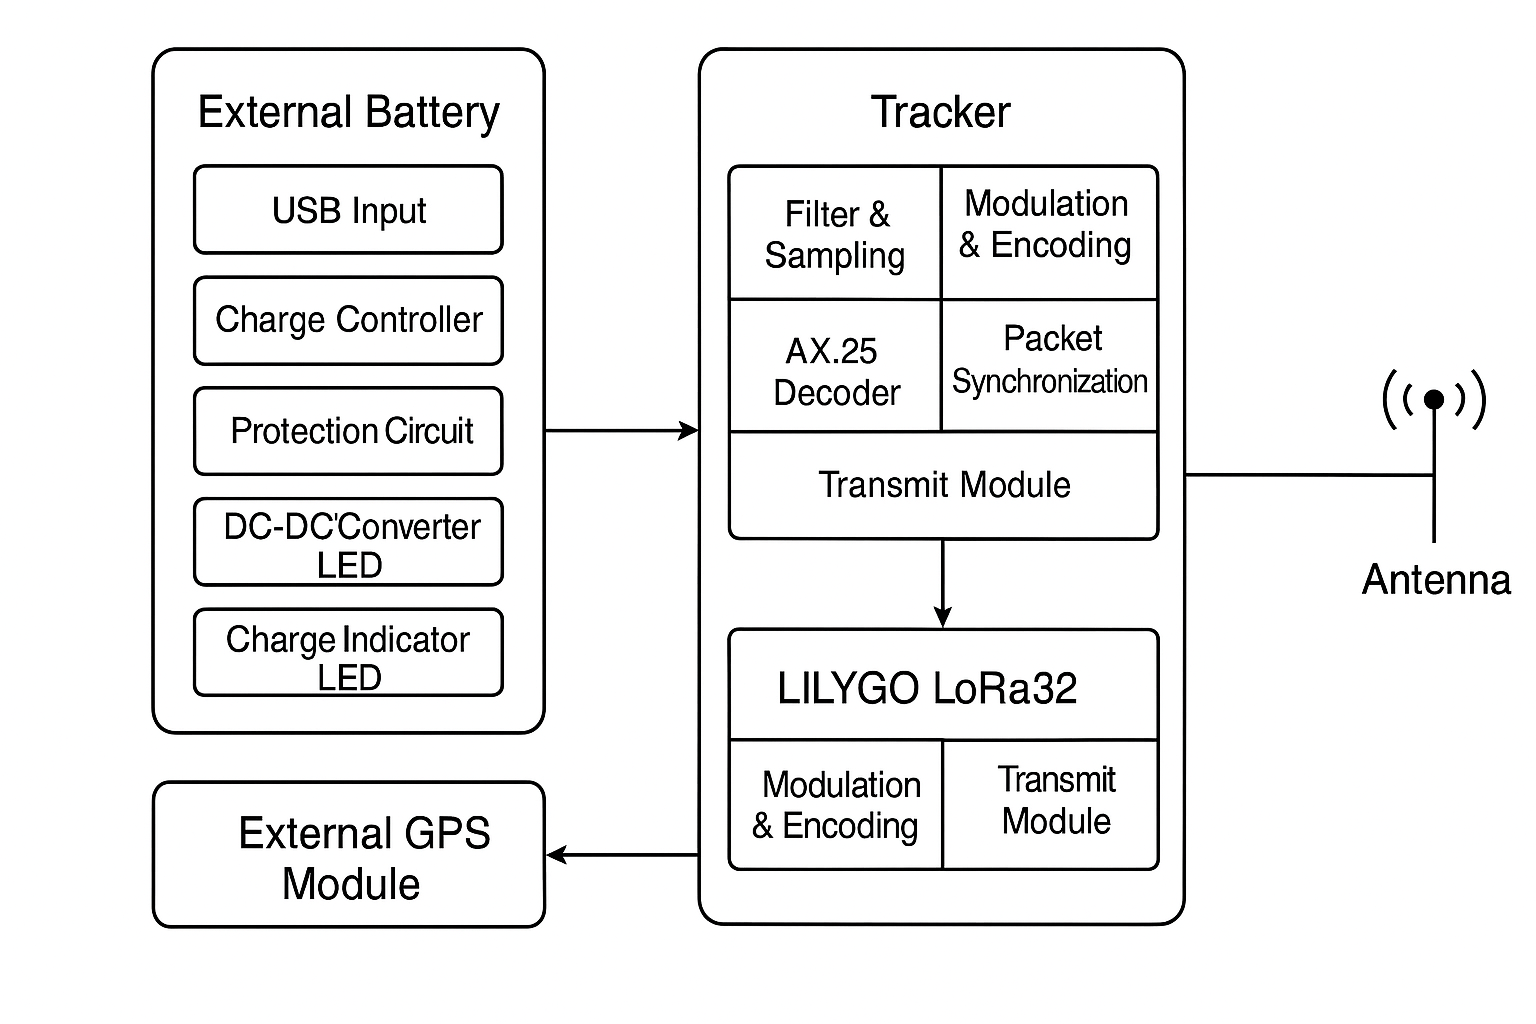
\includegraphics[width=0.4\textwidth]{Imagenes/tracker.png}
    \caption{Diagrama de bloques del sistema de rastreo}
    \label{fig:tracker}
\end{figure}

\vspace{2mm}

\subsection{Fuente de Energía (Batería Externa)}

Este bloque suministra energía al sistema de rastreo y está diseñado para ofrecer autonomía prolongada en ubicaciones remotas. Incorpora una entrada USB para recarga, un controlador de carga que regula y protege el proceso, celdas de almacenamiento, un circuito de protección ante condiciones adversas, un convertidor DC-DC para ajustar el voltaje de salida, y un LED indicador del estado de carga. Este sistema garantiza un suministro energético continuo, vital para el funcionamiento sostenido del tracker.

\vspace{2mm}

\subsection{Módulo GPS Externo}

Este módulo se encarga de determinar la localización del animal u objeto rastreado. Utiliza recepción satelital para obtener coordenadas geográficas precisas, las cuales se transmiten en formato NMEA (National Marine Electronics Association), estándar ampliamente aceptado que facilita su interpretación por el sistema. Esta información es crucial para analizar desplazamientos y patrones de comportamiento.

\vspace{2mm}

\subsection{Unidad Central de Rastreo (Tracker)}

\subsubsection*{ESP32}

El microcontrolador ESP32 actúa como el núcleo del sistema. Integra funciones clave como la adquisición y filtrado de datos, garantizando precisión en la información de posición y variables ambientales. Además, incluye un decodificador AX.25 que permite la compatibilidad con redes APRS, y un gestor de interrupciones que asegura la respuesta a eventos críticos como pérdida de señal o fallos energéticos. Este bloque es responsable de procesar toda la información previa a su transmisión.

\vspace{2mm}

\subsubsection*{LILYGO LoRa32}

\vspace{2mm}

Este componente es el encargado de la comunicación del sistema mediante tecnología LoRa. Incluye mecanismos de modulación y codificación que refuerzan la integridad de los datos ante interferencias, sincronización de paquetes para asegurar el orden correcto de transmisión, y un módulo transmisor que envía la información recolectada a través de una antena. Todo esto se realiza con un consumo energético mínimo, ideal para entornos con escasa infraestructura.


\newpage


\begin{thebibliography}{20}
 
	%Each item starts with a \bibitem{} command and the details thereafter.

    \bibitem{APRS} APRS Foundation, \textit{Automatic Packet Reporting System}, URL: \url{https://www.aprs.org/}.
    
    \bibitem{LoRa} Rcarrillo. (2024, July 24). Qué es LoRa, cómo funciona y características principales. Venco Electrónica. URL: \url {https://www.vencoel.com/que-es-lora-como-funciona-y-caracteristicas-principales/}

    \bibitem{PNAF} González, E. (2023). ALCA99\_30\_05\_2023 Reforma integral PNAF. Recuperado el 31 de mayo de 2023. URL: \url {https://sutel.go.cr/sites/default/files/normativas/Plan%20Nacional%20de%20Atribuicio%CC%81n%20de%20Frecuencias%20%28mayo%202023%29_0.pdf}


    \bibitem{paper} W. Chanwattanapong, S. Hongdumnuen, B. Kumkhet, S. Junon and P. Sangmahamad, "\textit{LoRa Network Based Multi-Wireless Sensor Nodes and LoRa Gateway for Agriculture Application}," 2021 Research, Invention, and Innovation Congress: Innovation Electricals and Electronics (RI2C), Bangkok, Thailand, 2021, pp. 133-136. 
    
 
    %%% The 1,2 etc. are used to cite in text. See up in the intro for an example
    %%% When you want to cite in your cite, type in \cite{} wherever you want
\end{thebibliography}



\end{document}